%%%%%%%%%%%%%%%%%%%%%%%%%%%%%%%%%%%%%%%%%%%%%%%%%%%%%%%%%%%%%%%%%%%%%%
%%  Copyright by Wenliang Du.                                       %%
%%  This work is licensed under the Creative Commons                %%
%%  Attribution-NonCommercial-ShareAlike 4.0 International License. %%
%%  To view a copy of this license, visit                           %%
%%  http://creativecommons.org/licenses/by-nc-sa/4.0/.              %%
%%%%%%%%%%%%%%%%%%%%%%%%%%%%%%%%%%%%%%%%%%%%%%%%%%%%%%%%%%%%%%%%%%%%%%

\newcommand{\commonfolder}{../../common-files}

\documentclass[11pt]{article}

\usepackage[most]{tcolorbox}
\usepackage{times}
\usepackage{epsf}
\usepackage{epsfig}
\usepackage{amsmath, alltt, amssymb, xspace}
\usepackage{wrapfig}
\usepackage{fancyhdr}
\usepackage{url}
\usepackage{verbatim}
\usepackage{fancyvrb}
\usepackage{adjustbox}
\usepackage{listings}
\usepackage{color}
\usepackage{subfigure}
\usepackage{cite}
\usepackage{sidecap}
\usepackage{pifont}
\usepackage{mdframed}
\usepackage{textcomp}
\usepackage{enumitem}
\usepackage{ctex}


% Horizontal alignment
\topmargin      -0.50in  % distance to headers
\oddsidemargin  0.0in
\evensidemargin 0.0in
\textwidth      6.5in
\textheight     8.9in 

\newcommand{\todo}[1]{
\vspace{0.1in}
\fbox{\parbox{6in}{TODO: #1}}
\vspace{0.1in}
}


\newcommand{\unix}{{\tt Unix}\xspace}
\newcommand{\linux}{{\tt Linux}\xspace}
\newcommand{\minix}{{\tt Minix}\xspace}
\newcommand{\ubuntu}{{\tt Ubuntu}\xspace}
\newcommand{\setuid}{{\tt Set-UID}\xspace}
\newcommand{\openssl} {\texttt{openssl}}


\pagestyle{fancy}
\lhead{\bfseries SEED Labs}
\chead{}
\rhead{\small \thepage}
\lfoot{}
\cfoot{}
\rfoot{}


\definecolor{dkgreen}{rgb}{0,0.6,0}
\definecolor{gray}{rgb}{0.5,0.5,0.5}
\definecolor{mauve}{rgb}{0.58,0,0.82}
\definecolor{lightgray}{gray}{0.90}


\lstset{%
  frame=none,
  language=,
  backgroundcolor=\color{lightgray},
  aboveskip=3mm,
  belowskip=3mm,
  showstringspaces=false,
%  columns=flexible,
  basicstyle={\small\ttfamily},
  numbers=none,
  numberstyle=\tiny\color{gray},
  keywordstyle=\color{blue},
  commentstyle=\color{dkgreen},
  stringstyle=\color{mauve},
  breaklines=true,
  breakatwhitespace=true,
  tabsize=3,
  columns=fullflexible,
  keepspaces=true,
  escapeinside={(*@}{@*)}
}

\newcommand{\newnote}[1]{
\vspace{0.1in}
\noindent
\fbox{\parbox{1.0\textwidth}{\textbf{Note:} #1}}
%\vspace{0.1in}
}


%% Submission
\newcommand{\seedsubmission}{You need to submit a detailed lab report, with screenshots,
to describe what you have done and what you have observed.
You also need to provide explanation
to the observations that are interesting or surprising.
Please also list the important code snippets followed by
explanation. Simply attaching code without any explanation will not
receive credits.}

%% Book
\newcommand{\seedbook}{\textit{Computer \& Internet Security: A Hands-on Approach}, 2nd
Edition, by Wenliang Du. See details at \url{https://www.handsonsecurity.net}.}

%% Videos
\newcommand{\seedisvideo}{\textit{Internet Security: A Hands-on Approach},
by Wenliang Du. See details at \url{https://www.handsonsecurity.net/video.html}.}

\newcommand{\seedcsvideo}{\textit{Computer Security: A Hands-on Approach},
by Wenliang Du. See details at \url{https://www.handsonsecurity.net/video.html}.}

%% Lab Environment
\newcommand{\seedenvironment}{This lab has been tested on our pre-built
Ubuntu 16.04 VM, which can be downloaded from the SEED website.}






\newcommand{\seedlabcopyright}[1]{
\vspace{0.1in}
\fbox{\parbox{6in}{\small Copyright \copyright\ {#1}\ \ by Wenliang Du.\\
      This work is licensed under a Creative Commons
      Attribution-NonCommercial-ShareAlike 4.0 International License.
      If you remix, transform, or build upon the material, 
      this copyright notice must be left intact, or reproduced in a way that is reasonable to
      the medium in which the work is being re-published.}}
\vspace{0.1in}
}





\newcommand{\pkiFigs}{./Figs}

\newcommand{\OpenSSL} {\texttt{OpenSSL}\xspace}
\newcommand{\pkiserver}{\texttt{bank32.com}\xspace}

\lhead{\bfseries SEED Labs -- PKI 实验}


\begin{document}

\begin{center}
{\LARGE 公钥基础设施 (PKI) 实验}
\end{center}

\seedlabcopyright{2018}



% *******************************************
% SECTION
% *******************************************
\section{概述}



公钥密码学是当今安全通信的基础。
但是当通信的一方将其公钥发送给另一方时,会受到中间人的攻击。
根本的问题是,验证公钥的所有权不是一个容易解决的问题。
也就是给定公钥及其声明的所有者信息,我们如何确保公钥确实由声明的所有者拥有?
公钥基础设施(PKI)就是解决此问题的一种方法。


该实验的目的是让学生获得有关 PKI 的第一手经验。
SEED labs 有一系列关于公钥加密的实验,而这个实验则针对 PKI 。
通过完成本实验中的任务,学生应该能够更好地理解 PKI 的工作原理,
了解如何使用 PKI 保护 Web 以及如何用 PKI 抵御中间人攻击。
此外,学生将能够了解公钥基础设施中信任的根源,以及如果信任根被破坏,将会出现哪些问题。
本实验涵盖以下主题:

\begin{itemize}[noitemsep]
   \item 公钥加密与公钥基础设施(PKI)
   \item 证书颁发机构(CA)、X.509 证书和根 CA
   \item Apache, HTTP, 和 HTTPS
   \item 中间人攻击
\end{itemize}



\paragraph{阅读材料}
有关PKI的详细信息,请阅读以下内容:

\begin{itemize}
\item Chapter 23 of the SEED Book, \seedbook
\end{itemize}


\paragraph{相关实验}

与本实验相关的一个话题是基于PKI的传输层安全(TLS)。我们有一个单独的TLS实验。
另外,还有一个 \textit{RSA公钥加密和签名实验},其重点是公钥加密的算法部分。


\paragraph{实验环境} \seedenvironmentB


% *******************************************
% SECTION
% *******************************************
\section{实验环境}

在本实验中,我们将生成公钥证书,然后使用它们来保护 Web 服务器。
证书生成任务将在虚拟机上执行,但是我们将使用容器托管 Web 服务器。

\paragraph{容器安装及其命令}
%%%%%%%%%%%%%%%%%%%%%%%%%%%%%%%%%%%%%%%%%%%%
Please download the
\texttt{Labsetup.zip} file to your VM from the lab's website,
unzip it, enter the \texttt{Labsetup} folder, and 
use the \texttt{docker-compose.yml} file to 
set up the lab environment. Detailed explanation
of the content in this file and all the involved 
\texttt{Dockerfile} can be found from the 
user manual, which is linked to the website of this lab.
If this is the first time you set up a SEED lab environment
using containers, it is very important that you read 
the user manual. 

In the following, we list some of the commonly
used commands related to Docker and Compose. 
Since we are going to use 
these commands very frequently, we have created aliases for them
in the \texttt{.bashrc} file (in our provided SEEDUbuntu 20.04 VM).


\begin{lstlisting}
$ docker-compose build  # Build the container image
$ docker-compose up     # Start the container
$ docker-compose down   # Shut down the container

// Aliases for the Compose commands above
$ dcbuild       # Alias for: docker-compose build
$ dcup          # Alias for: docker-compose up
$ dcdown        # Alias for: docker-compose down
\end{lstlisting}


All the containers will be running in the background. To run
commands on a container, we often need to get a shell on
that container. We first need to use the \texttt{"docker ps"}  
command to find out the ID of the container, and then
use \texttt{"docker exec"} to start a shell on that 
container. We have created aliases for them in
the \texttt{.bashrc} file.

\begin{lstlisting}
$ dockps        // Alias for: docker ps --format "{{.ID}}  {{.Names}}" 
$ docksh <id>   // Alias for: docker exec -it <id> /bin/bash

// The following example shows how to get a shell inside hostC
$ dockps
b1004832e275  hostA-10.9.0.5
0af4ea7a3e2e  hostB-10.9.0.6
9652715c8e0a  hostC-10.9.0.7

$ docksh 96
root@9652715c8e0a:/#  

// Note: If a docker command requires a container ID, you do not need to 
//       type the entire ID string. Typing the first few characters will 
//       be sufficient, as long as they are unique among all the containers. 
\end{lstlisting}


If you encounter problems when setting up the lab environment, 
please read the ``Common Problems'' section of the manual
for potential solutions.


%%%%%%%%%%%%%%%%%%%%%%%%%%%%%%%%%%%%%%%%%%%%



\paragraph{DNS 设置}

在本文档中,我们以 \texttt{www.bank32.com} 为例说明如何部署具有此域名的 HTTPS Web 服务器。
学生需要使用其他名称完成实验。
除非教师额外指定名称,否则学生应在服务器名称中包括其姓氏和实验年份。
例如,王小二在 2020 年进行了此实验,
则服务器名称应为 \texttt{www.wang2020.com}。
你不需要拥有此域名,你只需要通过在 \texttt{/etc/hosts}
中添加以下条目即可将此名称映射到容器的IP地址
(第一个条目是必需的,否则,本实验说明中的示例将会失效):

\begin{lstlisting}
10.9.0.80   www.bank32.com
10.9.0.80   www.wang2020.com
\end{lstlisting}


% *******************************************
% SECTION
% *******************************************
\section{实验内容}


% -------------------------------------------
% SUBSECTION
% -------------------------------------------
\subsection{任务 1: 构建一个证书颁发机构(CA)}

证书颁发机构(CA)是颁发数字证书的一个受信任的实体。
数字证书通过证书指定的主体(Subject)证明公钥的所有权。
有许多商业化的CA被视为根CA。
在撰写本文时,VeriSign是最大的CA。
用户需要付费才能获得这些商业CA颁发的数字证书。


在这个实验中,我们需要创建数字证书,但是我们不会向任何商业CA付费。
我们会自己创建一个根CA,然后使用该CA为其他实体(例如服务器)颁发证书。
在此任务中,我们将自己设为根CA,并为此CA生成一个证书。
与通常由另一个CA签名的其他证书不同,根CA的证书是自签名的。
根CA的证书通常预加载到大多数操作系统,Web浏览器和其他依赖PKI的软件中。
根CA的证书是无条件信任的。


\paragraph{配置文件 {\tt openssl.conf}}
要使用 \OpenSSL 来创建证书,首先需要有一个配置文件。
配置文件的扩展名通常为 {\tt .cnf}。
在 \OpenSSL 的 {\tt ca}、 {\tt req} 和 {\tt x509} 命令中会使用到这个配置文件。
\texttt{openssl.conf} 的说明文档可以网络上找到,
\OpenSSL 默认会使用 \path{/usr/lib/ssl/openssl.cnf} 作为配置文件。
由于我们需要对这个文件做出一些改动,我们把它复制到当前目录,
并指定 \OpenSSL 使用这个副本。

配置文件中的 \texttt{[CA\_default]} 一节展示了我们需要准备的默认设置。
我们需要创建几个子目录。
请去掉 \texttt{unique\_subject} 一行的注释,以允许创建有相同主体的多张证书,
因为在这个实验中我们很可能遇到这种情况。

\begin{lstlisting}[caption={Default CA setting}]
[ CA_default ]
dir             = ./demoCA         # Where everything is kept
certs           = $dir/certs       # Where the issued certs are kept
crl_dir         = $dir/crl         # Where the issued crl are kept
database        = $dir/index.txt   # database index file.
#unique_subject = no               # Set to 'no' to allow creation of
                                    # several certs with same subject.
new_certs_dir   = $dir/newcerts    # default place for new certs.
serial          = $dir/serial      # The current serial number
\end{lstlisting}


对于 \texttt{index.txt} 文件, 创建一个空文件即可。
对于 \texttt{serial} ,放一个字符串格式的数(例如 1000)在文件中。
当你设置好了配置文件 \texttt{openssl.cnf} 之后就可以创建和颁发证书了。


\paragraph{证书颁发机构(CA)}
如前所述,我们需要为我们的CA生成一个自签名证书。
这意味着该CA是完全受信任的,并且其证书将用作根证书。
你可以运行以下命令为CA生成自签名证书:

\begin{lstlisting}
openssl req -x509 -newkey rsa:4096 -sha256 -days 3650 \
            -keyout ca.key -out ca.crt
\end{lstlisting}

系统将提示你输入一个密码。
不要丢失此密码,因为每次要使用此CA为其他人签名证书时,都必须输入密码。
它还将要求填写证书主体信息,例如“国家名称”“通用名称”等。
命令的输出存储在两个文件中:{\tt ca.key} 和 {\tt ca.crt}。
文件{\tt ca.key}包含CA的私钥,而{\tt ca.crt}包含公钥证书。


你也可以在命令行中指定主体信息和密码,这样就不会提示你输入任何其他信息。
在以下命令中,我们使用 \texttt{-subj} 设置主体信息;
使用 \texttt{-passout pass:dees} 将密码设置为 \texttt{dees} 。

\begin{lstlisting}
openssl req -x509 -newkey rsa:4096 -sha256 -days 3650 \
            -keyout ca.key -out ca.crt  \
            -subj "/CN=www.modelCA.com/O=Model CA LTD./C=US" \
            -passout pass:dees
\end{lstlisting}


我们可以使用以下命令查看 X509 证书和 RSA 密钥的解码内容
( \texttt{-text} 表示将内容解码为纯文本; \texttt{-noout} 表示不打印出编码版本):

\begin{lstlisting}
openssl x509 -in ca.crt -text -noout
openssl rsa  -in ca.key -text -noout
\end{lstlisting}

请运行以上命令,并从输出中找出以下内容:

\begin{itemize}[noitemsep]
   \item 证书中的哪一部分说明了这是一个 CA 的证书?
   \item 证书中的哪一部分说明了这是一个自签名证书?
   \item 在 RSA 算法中,我们有公开指数 $e$ 、私有指数 $d$、模数 $n$
         以及两个秘密的数 $p$ 和 $q$ 使得 $n = pq$ 。
         请从你的证书和密钥文件中找出这些元素的值。
\end{itemize}


% -------------------------------------------
% SUBSECTION
% -------------------------------------------
\subsection{任务 2: 为你的 Web 服务器生成证书请求}

生成证书签名请求(CSR)的命令与在创建 CA 自签名证书时使用的命令非常相似,
唯一的区别是是否带有 \texttt{-x509} 选项。
没有这个选项,该命令将生成一个证书签发请求;
加上这个选项,该命令将生成一个自签名证书。
以下命令为 \texttt{www.bank32.com} 生成 CSR (您应该使用自己的服务器名称):

\begin{lstlisting}
openssl req -newkey rsa:2048 -sha256  \
            -keyout server.key   -out server.csr  \
            -subj "/CN=www.bank32.com/O=Bank32 Inc./C=US" \
            -passout pass:dees
\end{lstlisting}

该命令将生成一对公私钥对,然后使用公钥创建证书签名请求。
我们可以使用以下命令查看 CSR 和私钥文件的解码内容:

\begin{lstlisting}
openssl req -in server.csr -text -noout
openssl rsa -in server.key -text -noout
\end{lstlisting}

\paragraph{添加备用名称(Alternative Name)}
许多网站都有不同的 URL 。
例如, \texttt{www.example.com} , \texttt{example.com} , \texttt{example.net}
和 \texttt{example.org} 都指向同一 Web 服务器。
由于浏览器实施了主机名匹配策略,因此证书中的公用名(Common Name)必须与服务器的主机名匹配,
否则浏览器将拒绝与服务器通信。

为了使证书具有多个名称, X.509 规范定义了一个可以附加到证书的扩展,名为主体备用名称(SAN)。
使用 SAN 扩展名,可以在证书的 \texttt{subjectAltName} 字段中指定多个主机名。

要使用此类字段生成证书签名请求,我们可以将所有必要的信息放在配置文件中或命令行中。
我们在本任务中使用命令行的方法(在 TLS 实验中会使用配置文件的方法)。
我们可以在 \texttt{openssl req} 命令中添加以下选项。
应当注意, \texttt{subjectAltName} 扩展字段还必须包括通用名称字段中的主机名。
否则,通用名称将不会被接受为有效名称。

\begin{lstlisting}
-addext "subjectAltName = DNS:www.bank32.com,  \
                          DNS:www.bank32A.com, \
                          DNS:www.bank32B.com"
\end{lstlisting}

请在你的证书签名请求中添加两个备用名称。
在后面的任务中将会用到它们。


% -------------------------------------------
% SUBSECTION
% -------------------------------------------
\subsection{任务 3: 为你的服务器生成证书}

CSR文件需要具有CA的签名才能形成证书。
在现实世界中,通常将CSR文件发送到受信任的CA进行签名。
在本实验中,我们将使用我们自己的受信任CA生成证书。
以下命令使用CA的 {\tt ca.crt} 和 {\tt ca.key} ,
将证书签名请求( {\tt server.csr} )转换为X509证书({\tt server.crt}):

\begin{lstlisting}
openssl ca -config myCA_openssl.cnf -policy policy_anything \
            -md sha256 -days 3650 \
            -in server.csr -out server.crt -batch \
            -cert ca.crt -keyfile ca.key
\end{lstlisting}

在上面的命令中,\texttt{myCA\_openssl.cnf} 是我们从 \path{/usr/lib/ssl/openssl.cnf}
复制的配置文件(我们在任务 1 中对此文件进行了更改)。
我们使用配置文件中定义的 \texttt{policy\_anything} 策略,这不是默认策略。
默认策略有更多限制,要求请求中的某些主体信息必须与 CA 证书中的主体信息匹配。
命令中使用的策略不强制执行任何匹配规则。

\paragraph{复制扩展域}
出于安全原因,\texttt{openssl.cnf} 中的默认设置
不允许 \texttt{openssl ca} 命令将扩展字段从请求复制到最终证书。
为此,我们可以在配置文件的副本中,取消以下行的注释:

\begin{lstlisting}
# Extension copying option: use with caution.
copy_extensions = copy
\end{lstlisting}

签署证书后,请使用以下命令输出证书的解码内容,并检查是否包含备用名称。

\begin{lstlisting}
openssl x509 -in server.crt -text -noout
\end{lstlisting}



% -------------------------------------------
% SUBSECTION
% -------------------------------------------
\subsection{任务 4: 在基于Apache的HTTPS网站中部署证书}

在此任务中,我们将看到网站如何使用公钥证书来保护 Web 浏览。
我们将建立一个基于 Apache 的 HTTPS 网站。
我们的容器中已经安装了 Apache 服务器,它支持 HTTPS 协议。
要搭建 HTTPS 网站,我们只需要配置 Apache 服务器,让它知道从哪里获取私钥和证书。
在容器内部,我们已经为 \pkiserver 设置了 HTTPS 站点。
学生可以按照以下示例来设置自己的 HTTPS 网站。

一个Apache服务器可以同时托管多个网站。
它需要知道网站文件的存储目录。
这是通过位于 \url{/etc/apache2/sites-available} 目录中的 \texttt{VirtualHost} 文件完成的。
在我们的容器中,我们有一个名为 \texttt{bank32\_apache\_ssl.conf} 的文件,其中包含以下条目:

\begin{lstlisting}
<VirtualHost *:443>
   DocumentRoot /var/www/bank32
   ServerName www.bank32.com
   ServerAlias www.bank32A.com
   ServerAlias www.bank32B.com
   DirectoryIndex index.html
   SSLEngine On
   SSLCertificateFile    /certs/bank32.crt    (*@\ding{192}@*)
   SSLCertificateKeyFile /certs/bank32.key    (*@\ding{193}@*)
</VirtualHost>
\end{lstlisting}

上面的示例设置了 HTTPS 站点 \url{https://www.bank32.com}
(端口 \texttt{443} 是默认的 HTTPS 端口)。
\texttt{ServerName} 条目指定网站的名称,
而 \texttt{DocumentRoot} 条目指定网站文件的存储位置。
使用 \texttt{ServerAlias} 条目,我们允许网站使用不同的名称。
你也应该提供两个别名条目。


我们还需要告诉 Apache 服务器证书(\ding{192})和私钥(\ding{193})的存储位置。
在 \texttt{Dockerfile} 中,我们已经包含了
用于将证书和密钥复制到容器的 \texttt{/certs}文件夹的命令。

为了使该网站正常工作,我们需要启用 Apache 的 \texttt{ssl} 模块,然后启用该网站。
可以使用以下命令完成操作,这些命令在构建容器时已经执行。

\begin{lstlisting}
# a2enmod ssl                 // Enable the SSL module
# a2ensite bank32_apache_ssl  // Enable the sites described in this file
\end{lstlisting}



\paragraph{启动 Apache 服务器}
在容器中 Apache 服务器不会自动启动。
我们需要在容器里运行以下命令来启动服务器(我们还列出了一些相关命令):

\begin{lstlisting}
// Start the server
# service apache2 start

// Stop the server
# service apache stop

// Restart a server
# service apache restart
\end{lstlisting}

Apache 启动时,需要为每个 HTTPS 站点加载私钥。
我们的私钥已加密,因此 Apache 会要求我们输入密码进行解密。
在容器内,用于 \texttt{bank32} 的密码为 \texttt{dees} 。
如果一切设置正确,我们就可以浏览该网站,并且浏览器和服务器之间的所有流量都将被加密。

请使用以上示例作为指导,为您的网站设置 HTTPS 服务器。
请描述你的操作步骤、添加到 Apache 的配置文件中的内容以及最终结果的屏幕快照,
以展示你可以成功浏览 HTTPS 站点。

\paragraph{浏览网站}
现在,用浏览器访问你的 Web 服务
(注意:你应该在 URL 的开头加上 \texttt{https},而不要使用 \texttt{http})。
请描述你观察到的现象并做出解释。
您很可能无法成功,这是因为……(此处省略了原因,学生应在实验报告中做出解释)。
请解决此问题,并证明你可以成功访问 HTTPS 网站。

下面,我们说明如何将证书加载到 Firefox 。
学生需要自己弄清楚为什么以及应该加载什么证书。
要将证书手动添加到 Firefox 浏览器,请在地址栏中键入以下URL,
然后单击页面上的 \texttt{View Certificates} 按钮(滚动到底部)。

\begin{lstlisting}
about:preferences#privacy
\end{lstlisting}

在 \texttt{Authorities} 标签中,你将看到已被 Firefox 接受的证书列表。
在这里,我们可以导入我们自己的证书。
选择证书文件后,请选择 ``Trust this CA to identify websites'' 选项。
你会看到我们的证书现在在 Firefox 接受的证书列表中。



% -------------------------------------------
% SUBSECTION
% -------------------------------------------
\subsection{任务 5: 发起中间人攻击}

在此任务中,我们将展示 PKI 如何抵御中间人(MITM)攻击。
图 \ref{pki:fig:mitm} 描述了MITM攻击的工作方式。
假设 Alice 想通过HTTPS协议访问 \texttt{example.com}。
她需要从 \texttt{example.com} 服务器获取公钥; Alice 将生成一个秘密,并使用服务器的公钥对该秘密进行加密,然后将其发送到服务器。
如果攻击者可以拦截 Alice 与服务器之间的通信,那么攻击者可以用其自己的公钥替换服务器的公钥。
这样 Alice 的秘密实际上是使用攻击者的公钥加密的,因此攻击者将能够读取该秘密。
攻击者可以使用服务器的公钥将秘密转发给服务器。
因为该秘密将用于加密 Alice 和服务器之间的通信,因此攻击者可以解密加密的通信。


\begin{figure}[htb]
   \begin{center}
      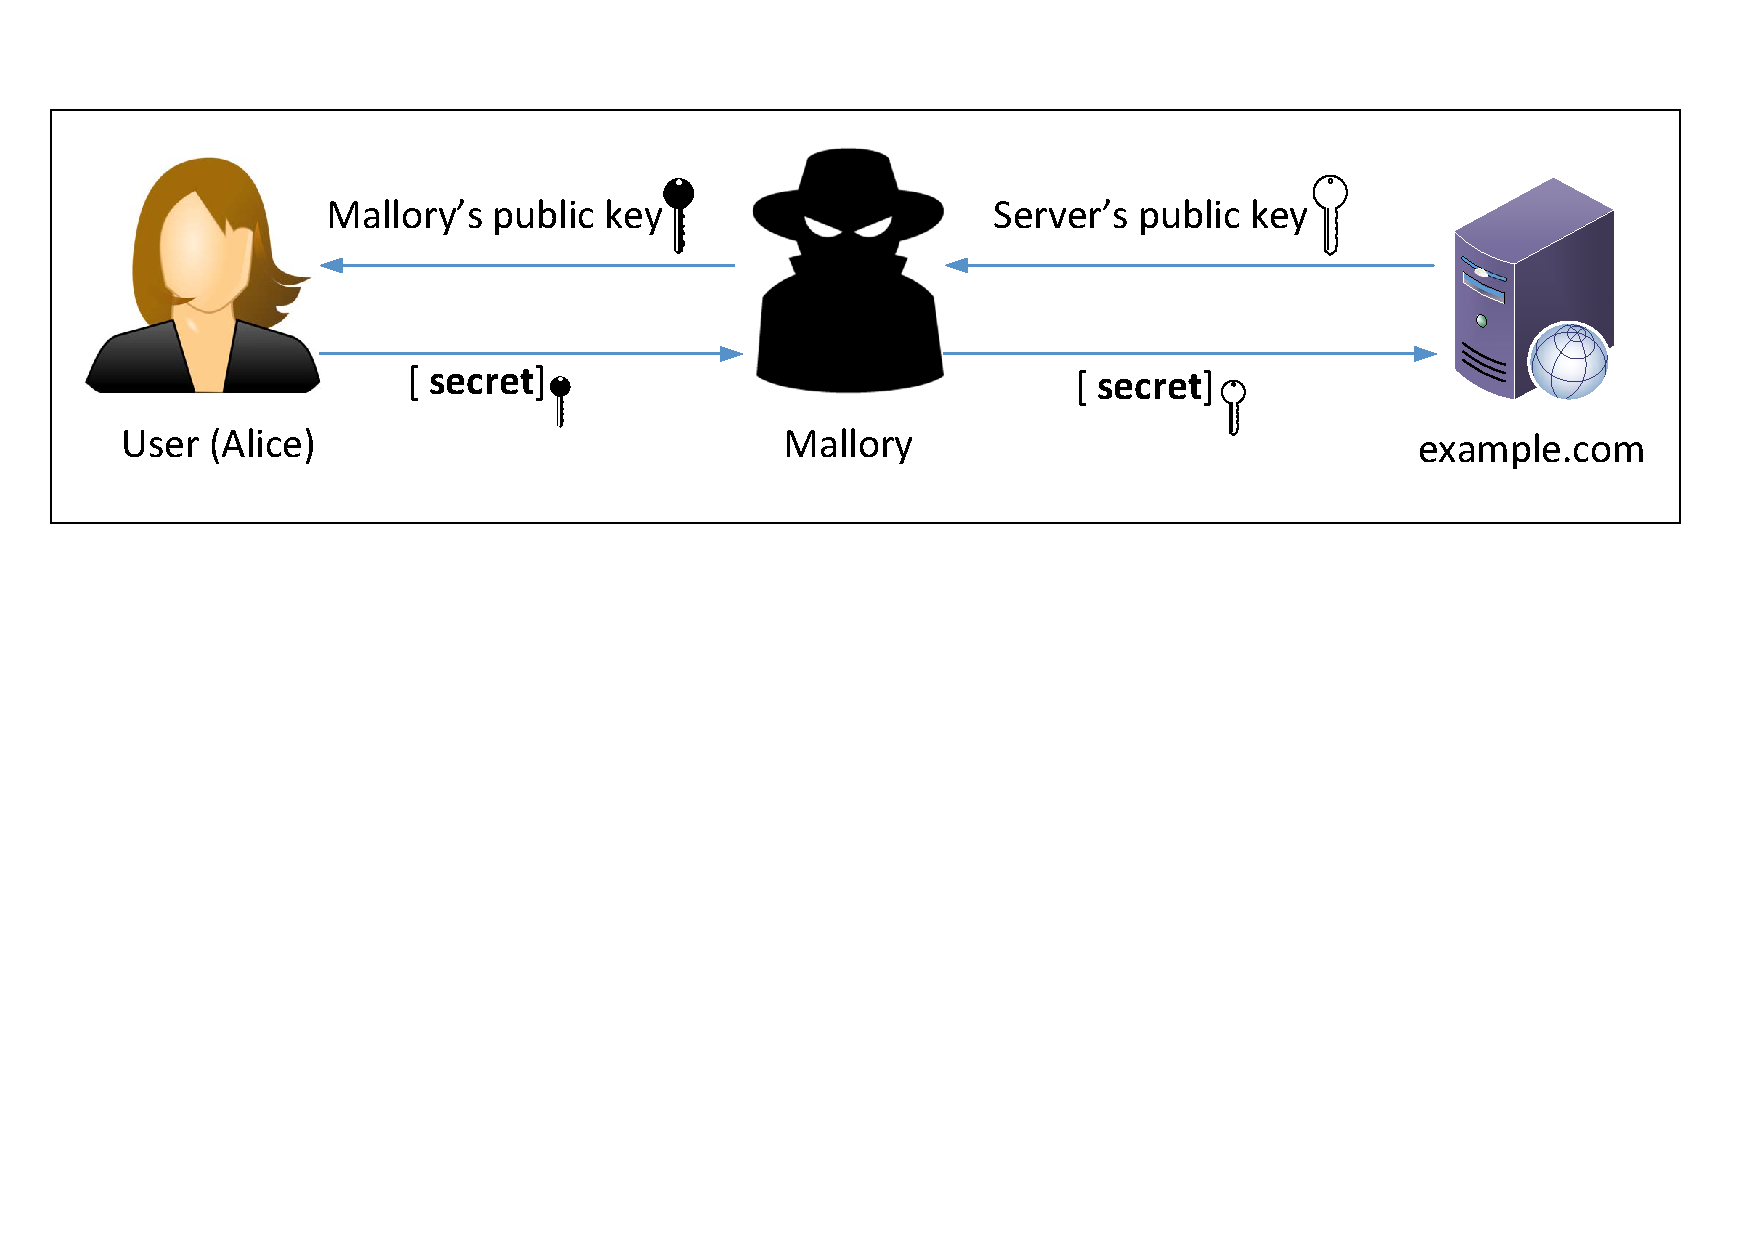
\includegraphics[width=0.8\textwidth]{\pkiFigs/mitm.pdf}
   \end{center}
   \caption{中间人攻击}
   \label{pki:fig:mitm}
\end{figure}


该任务的目的是帮助学生了解 PKI 如何抵御此类MITM攻击。
在任务中,我们将模拟一次MITM攻击,并了解PKI如何精确地防御。
我们将首先选择一个目标网站。
在本文档中,我们使用 \texttt{example.com} 作为目标网站。
但在实际任务中,为了使其更有意义,学生可以选择一个受欢迎的网站,例如银行网站或者社交网站。


\paragraph{第 1 步: 启动一个恶意网站}
在任务4中,我们已经为 \pkiserver 建立了HTTPS网站。
我们将使用同一台 Apache 服务器来模拟 \texttt{www.example.com} (或学生选择的站点)。
为此,我们将按照任务4中的说明向Apache的SSL配置文件中添加 \texttt{VirtualHost} 条目,
\texttt{ServerName} 应该为 \texttt{example.com} ,
但其余配置可以与任务4中使用的相同。
显然在真实世界中你不可能获得一个 \texttt{www.example.com} 的合法证书,
所以我们将会使用与我们自己的服务器相同的证书。


我们的目标如下:当用户尝试访问 \texttt{example.com} 时,
我们将使该用户进入我们的服务器,该服务器托管一个伪造的 \texttt{example.com}。
如果这是一个社交网络网站,则假网站可以显示类似于目标网站中的登录页面。
如果用户无法分辨出区别,则可以在伪造的网页中键入其帐户凭据,从而使攻击者获得凭据。


\paragraph{第 2 步: 成为中间人}
有几种方法可以使用户的 HTTPS 请求进入我们的 Web 服务器。
一种方法是路由攻击,使用户的 HTTPS 请求被路由到我们的 Web 服务器。
另一种方法是 DNS 攻击,当受害者的计算机尝试找出目标 Web 服务器的 IP 地址时,
它将获取到我们 Web 服务器的 IP 地址。
在此任务中,我们模拟 DNS 攻击。
我们无需发动真正的的 DNS 缓存中毒攻击,只需要修改受害者机器的 \texttt{/etc/hosts} 文件,
通过把 \texttt{www.example.com} 映射到
我们的恶意 Web 服务器上来模拟 DNS 缓存存储攻击的结果。


\begin{lstlisting}
10.9.0.80  www.example.com
\end{lstlisting}


\paragraph{第 3 步: 浏览目标网站}
完成所有设置后,现在访问目标真实网站,并查看您的浏览器会说些什么。
请解释你观察到的现象。



% -------------------------------------------
% SUBSECTION
% -------------------------------------------
\subsection{任务 6: 使用一个被攻陷的 CA 发起中间人攻击}

在本任务中,假设我们在任务 1 中创建的根 CA 被攻击者攻破,并且其私钥被盗。
因此,攻击者可以使用此 CA 的私钥生成任意证书。
在此任务中,我们将看到这种破坏的结果。



请设计一个实验,以表明攻击者可以在任何HTTPS网站上成功发起MITM攻击。
你可以使用在任务5中创建的相同设置,但是这次,你需要证明MITM攻击是成功的。
即当受害人试图访问网站时,浏览器不会有起任何怀疑,而是落入MITM攻击者的虚假网站。




% *******************************************
% SECTION
% *******************************************
\section{提交}

\seedsubmission


%%%%%%%%%%%%%%%%%%%%%%%%%%%%%%%%%%%%%%%%%%%%%%%%%%%%%%
\end{document}
%%%%%%%%%%%%%%%%%%%%%%%%%%%%%%%%%%%%%%%%%%%%%%%%%%%%%%

